\newpage

\section{Constant Propagation/Folding\cite{Microsof98:online}}


\subsection{Problem Definition }


Given a program, we would like to know for every point in the program (after every
statement), which variables have constant values, and which do not. We say that a
variable has a constant value at a certain point if every execution that reaches that point,
gives that variable the same constant value.


\subsection{Meet Operator}

\begin{figure}[H]
	\centering
	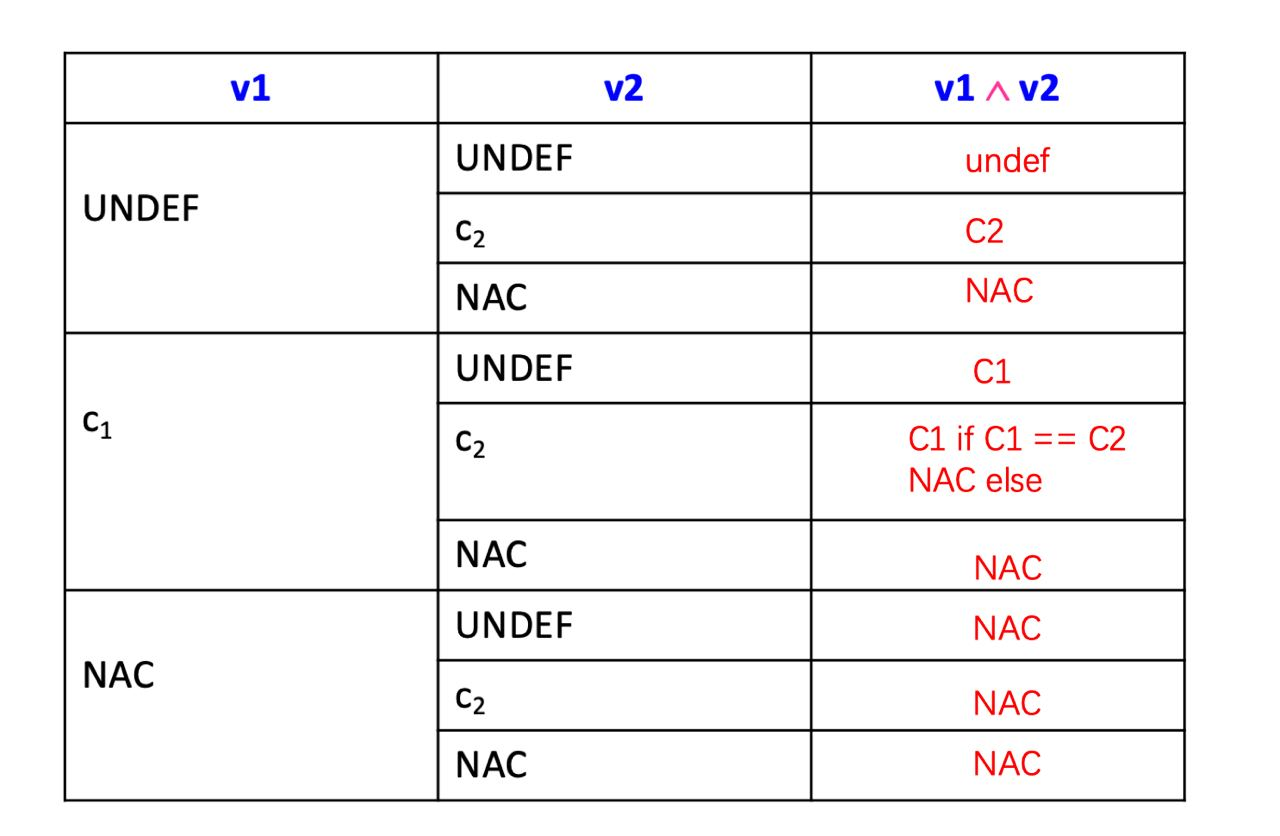
\includegraphics[width=0.6\textwidth]{p219.jpg}
	\caption{Meet operator for Constant Propagation.}
	\label{fig:p219}
\end{figure}


\subsection{Transfer Function}


Let an assignment be of the form $x_3 = x_1 + x_2$, $+$ represents a generic operator.


\begin{figure}[H]
	\centering
	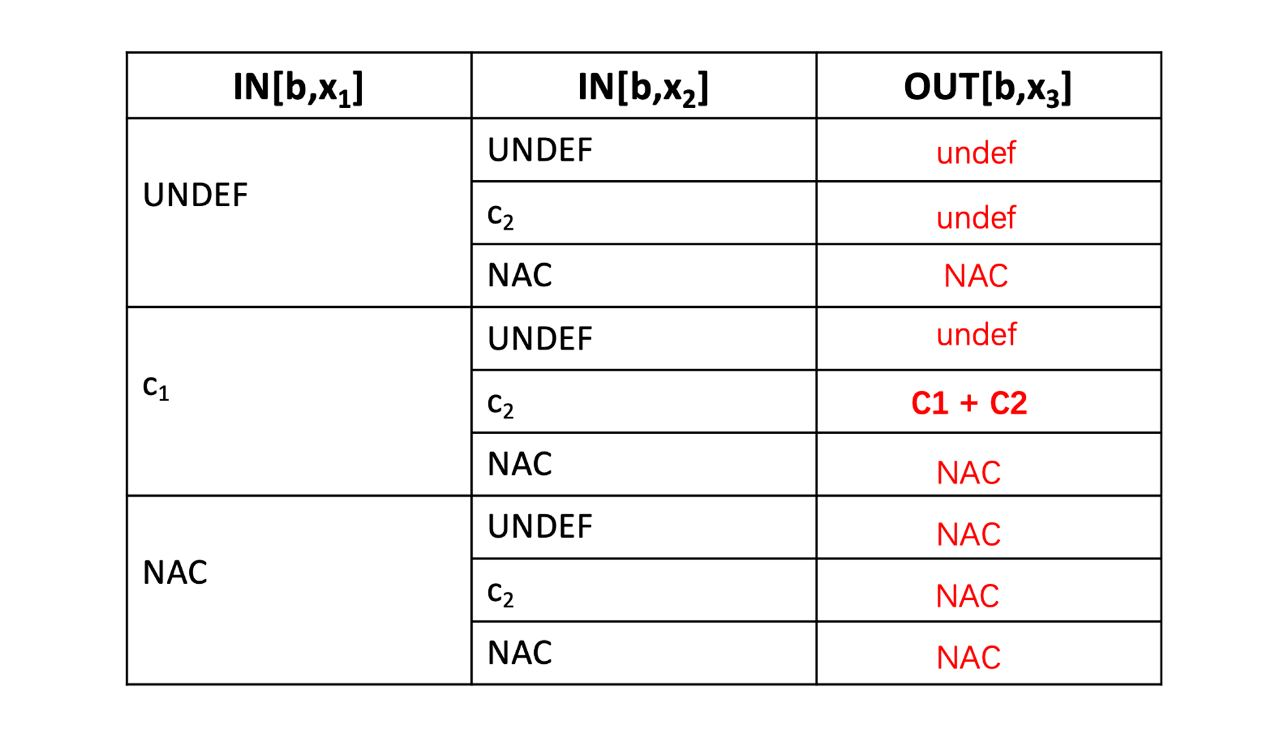
\includegraphics[width=0.6\textwidth]{p220.jpg}
	\caption{Transfer Function.}
	\label{fig:p220}
\end{figure}

\subsection{Summary}
Constant Propogation is not distributive\footnote{See Figure \ref{fig:p221}}.
The semi-lattice is shown in Figure \ref{fig:p222}.



\begin{figure}[H]
	\centering
	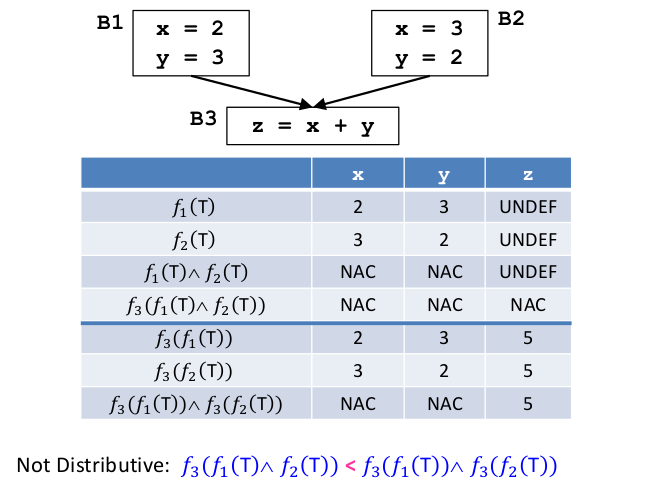
\includegraphics[width=0.6\textwidth]{p222.png}
	\caption{Constant Propogation is not Distributive.}
	\label{fig:p222}
\end{figure}


\begin{figure}[H]
	\centering
	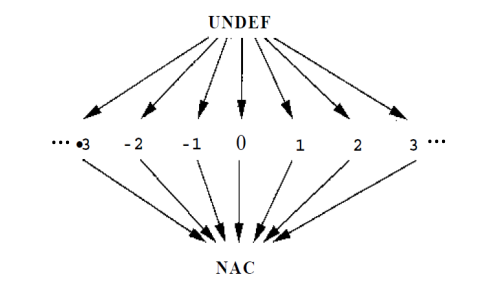
\includegraphics[width=0.6\textwidth]{p221.png}
	\caption{Constant Propogation's Semi-lattice Diagram.}
	\label{fig:p221}
\end{figure}


\begin{center}
	\begin{tabular}{|c|c|}
		\hline Direction                         & Forward                                \\
		\hline Domain                            & Numbers                                \\
		\hline Top(T)                          & $\mathrm{UNDEF}$                       \\
		\hline Bottom                            & $\mathrm{NAC}$                         \\
		\hline Boundary condition                & $\mathrm{OUT[ENTRY]} = \mathrm{UNDEF}$ \\
		\hline Initialization for internal nodes & $\mathrm{OUT[B]} = \mathrm{UNDEF}$     \\
		\hline Finited escending chain?          & \checkmark                             \\
		\hline Monotone ?                        & \checkmark                             \\
		\hline Distributive?                     & \text{\sffamily X}                             \\
		\hline
	\end{tabular}
\end{center}




